اطلاعات جمع آوری شده از سایت زیر است:
\\
 \begin{latin}
 \url{https://store.steampowered.com/}
 \end{latin}
 \\
با استفاده از کتابخانه \lr{BeautifulSoup} اطلاعات مورد نیاز از سایت \lr{crawl} شده است. به دلیل تعداد بالای رکوئست‌ها و پرشدن حافظه‌ی \lr{RAM} هر ۵ هزار داده در یک فایل ذخیره شده‌اند. اما در نهایت، اطلاعات مربوط به بازی‌های یک گروه، در یک فایل قرار داده شده‌اند.

روش کار به این صورت است که در ابتدا، لیست \lr{app\_id} مربوط به بازی های یک گروه را استخراج کرده، به کمک تابع \lr{add\_information} به تک تک \lr{app\_id}‌ها، رکوئست می‌فرستیم تا اطلاعات (نام و توضیحات) مربوط به بازی، به دست آید.
\\
کد:
\begin{figure}[H]
    \centering
    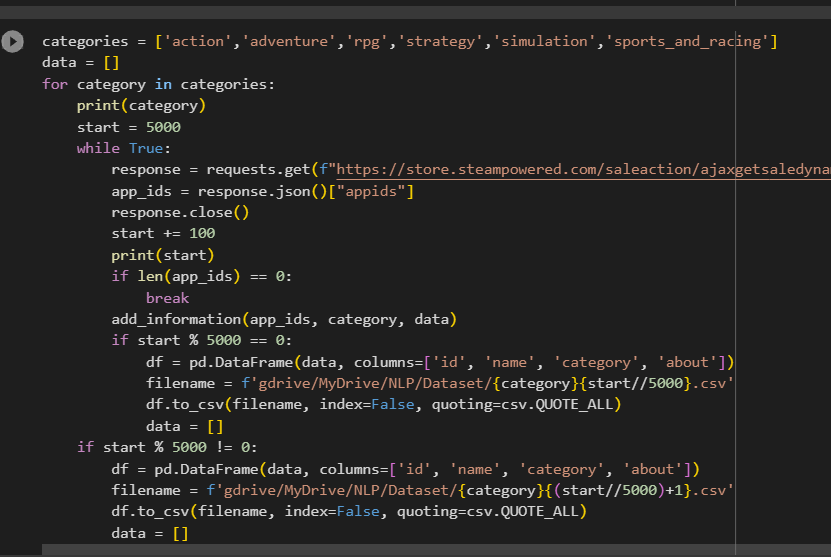
\includegraphics[width=0.7\linewidth]{./images/c_code1.png}
   \end{figure}


\begin{figure}[H]
    \centering
    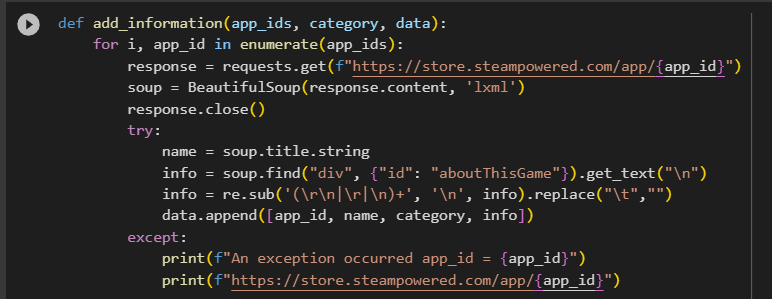
\includegraphics[width=0.7\linewidth]{./images/c_code2.png}
   \end{figure}

\begin{figure}[H]
    \centering
    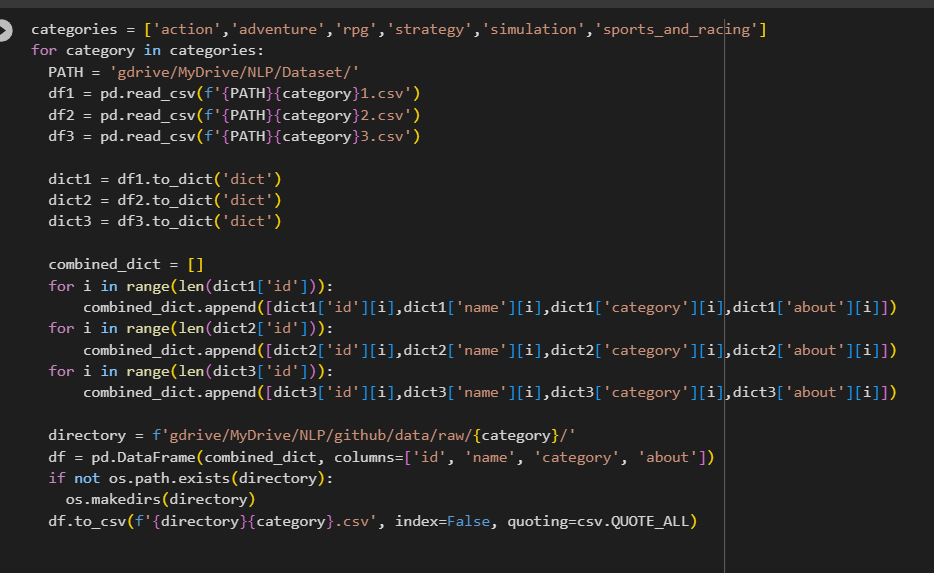
\includegraphics[width=0.7\linewidth]{./images/c_code3.png}
   \end{figure}


لیست اطلاعات بازی های مربوط به 6 گروه دراورده شده و اطلاعات هر گروه در فولدر مربوطه قرار گرفته شده است.
فرمت داده ها به شکل فایل .csv  هست.
\begin{figure}[H]
    \centering
    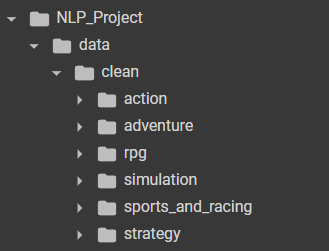
\includegraphics[width=0.4\linewidth]{./images/files.png}
   \end{figure}
   
برای تفکیک جملات و کلمات، از متدهای موجود در کتابخانه nltk استفاده کردم. این متدها شامل توابعی مانند sent\_tokenize() برای تفکیک جملات و word\_tokenize() برای تفکیک کلمات هستند.
\begin{figure}[H]
    \centering
    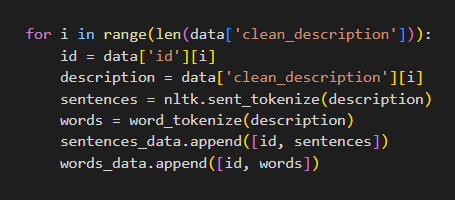
\includegraphics[width=0.7\linewidth]{./images/e_code1.png}
   \end{figure}
   
\newpage

برای  بخش clean کردن داده،  ابتدا عبارت \lr{"About the game"} را از ابتدای متن حذف کرده و سپس بررسی کرده‌ایم که آیا توضیحات بازی کمتر از ده حرف هستند؟ در صورتی که چنین باشد، آن‌ها را نیز حذف می‌کنیم.

\begin{figure}[H]
    \centering
    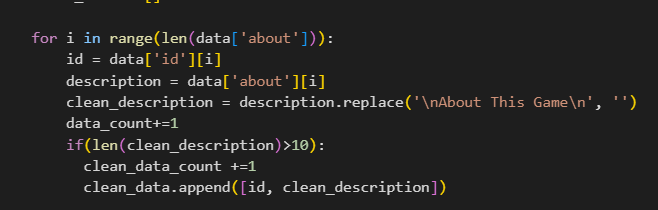
\includegraphics[width=0.7\linewidth]{./images/e_code2.png}
   \end{figure}

\\
تعداد داده قبل و بعد از clean  کردن :

\begin{figure}[H]
    \centering
    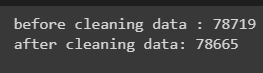
\includegraphics[width=0.7\linewidth]{./images/b_a_clean.png}
   \end{figure}
   \\
   
واحد برچسب گذاری برای هر متن بازی ، ژانر خود بازی هست. برای مثال اگر ژانر بازی اکشن باشند برچسب توضیحات آن ، اکشن می‌شود.

آمار داده به تفکیک برچسب در قالب جدول «و» نمودار
\\
أ. تعداد «واحد» داده
\begin{latin}
\begin{center}
  \fontsize{8pt}{9pt}\ttfamily
  \csvautotabular[respect all]{../stats/data_count.csv}
\end{center}
\end{latin}

\\
ب. تعداد جملات
\begin{latin}
\begin{center}
  \fontsize{8pt}{9pt}\ttfamily
  \csvautotabular[respect all]{../stats/sentences_count.csv}
\end{center}
\end{latin}

\\
\newpage
ج. تعداد کلمات
\begin{latin}
\begin{center}
  \fontsize{8pt}{9pt}\ttfamily
  \csvautotabular[respect all]{../stats/words_count.csv}
\end{center}
\end{latin}

\\

د. تعداد کلمات منحصر به فرد

\

\begin{latin}
\begin{center}
  \fontsize{8pt}{9pt}\ttfamily
  \csvautotabular[respect all]{../stats/unique_common_uncommon_count.csv}
\end{center}
\end{latin}

ه. تعداد کلمات منحصر به فرد مشترک و غیر مشترک بین برچسب ها
\begin{latin}
\begin{center}
  \fontsize{8pt}{9pt}\ttfamily
  \csvautotabular[respect all]{../stats/unique_common_uncommon_count.csv}
\end{center}
\end{latin}

\newpage

و.  ۱۰کلمه پرتکرار غیر مشترک هر برچسب
\begin{latin}
\begin{center}
    \fontsize{4pt}{7pt}\ttfamily
  \csvautotabular[respect all]{../stats/ten_uncommon_words.csv}
\end{center}
\end{latin}

ز.  ۱۰کلمه مشترک برتر هر برچسب نسبت به برچسبهای دیگر بر اساس معیار زیر
\begin{latin}
\begin{center}
  \fontsize{4pt}{7pt}\ttfamily
  \csvautotabular[respect all]{../stats/ten_common_words.csv}
\end{center}
\end{latin}


ح. ده کلمه برتر بر اساس \lr{TF\_IDF(W)}
\begin{latin}
\begin{center}
  \fontsize{4pt}{7pt}\ttfamily
  \csvautotabular[respect all]{../stats/ten_common_words.csv}
\end{center}
\end{latin}


\newpage

ط. هیستوگرام تعداد تکرار هر کلمه منحصر به فرد به ترتیب از فرکانس بالا به پایین
\begin{figure}[H]
    \centering
    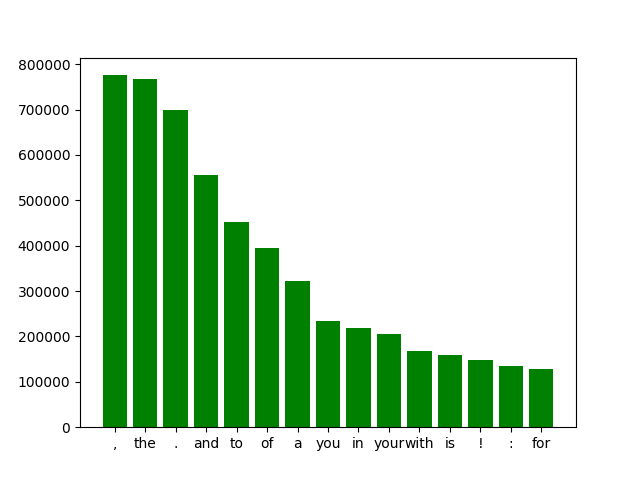
\includegraphics[width=0.7\linewidth]{../stats/hist.png}
   \end{figure}
   
لینک \lr{github} :
\\
 \begin{latin}
 \url{ https://github.com/bavanDA/NLP\_Project}
 \end{latin}
 

\\
لینک \lr{huggingface}:
\\
 \begin{latin}
 \url{https://huggingface.co/datasets/Bavanda/Steam\_DG}
 \end{latin}
 
